
%
%  $Description: Application Scheduling in CloudSim$ 
%
%  $Author: Pradeeban $
%  $Date: 2013/11/20 17:04:59 $
%  $Revision: 1.4 $
%

\documentclass[times, 10pt,twocolumn]{article} 
\usepackage{cloudsim}
\usepackage{times}
\usepackage{moreverb}
\usepackage{amsmath}
\usepackage{graphicx}     % to include images
\usepackage[utf8]{inputenc}
\usepackage[T1]{fontenc}

%\documentstyle[times,art10,twocolumn,cloudsim]{article}

%------------------------------------------------------------------------- 
% take the % away on next line to produce the final camera-ready version 
\pagestyle{empty}

%------------------------------------------------------------------------- 
\begin{document}

\title{Application Scheduling in CloudSim}

\author{Pradeeban Kathiravelu\\
KTH Royal Institute of Technology, Stockholm, Sweden.\\ kpr@kth.se\\
}

\maketitle
\thispagestyle{empty}

\begin{abstract}
   Cloud Computing involves multiple users with multiple shared resources, such as processor, bandwidth, and memory. Many of the user submitted tasks require a considerable amount of resources to be allocated exclusively for them for a successful operation. Jobs should be scheduled in a timely manner to the available resources, for a successful and efficient execution. Many application scheduling algorithms are implemented to fairly schedule the jobs of the users to the available resources. Prior to test the scheduling algorithm in the real cloud environment, they are often tested on a simulation environment such as CloudSim or EmuSim. This paper looks into the three families of application scheduling algorithms -  Strict matchmaking-based, utility-driven, and QoS-driven algorithms, and evaluates them against multiple criteria to find their effectiveness. 
\end{abstract}


\textbf{Categories and Subject Descriptors}\\
D.2.8 \textbf{[Software Engineering]}: Operating Systems - scheduling\\
D.2.8 \textbf{[Software Engineering]}: Metrics - performance measures\\
\textbf{General Terms}\\
Simulation\\
\textbf{Keywords} -  Application Scheduling, Strict Matchmaking-based algorithms, Utility-driven algorithms, QoS-driven algorithms, Cloud Simulation, VM (Virtual Machine).

%------------------------------------------------------------------------- 
\Section{Introduction}

Application scheduling plays a major role in a system that has resources distributed and shared among multiple users. Fair scheduling of the resources is mandatory for the successful execution of the system. With the ever increasing complexity of the cloud environments such as the heterogeneity and geographic dispersion of the cloud resources, as well as the users submitting the applications from different geographic locations, scheduling the applications has become a harder task to accomplish, making it a promising research field.

Application scheduling in a cloud environment has to consider the geographically distributed user applications and the diverse computing resources such as the processor, memory, and bandwidth. Scheduling algorithms are developed to find a resource for any given job that fulfills the job requirements. Three families of algorithms are developed to address this, naming, strict matchmaking-based algorithms, utility-driven algorithms, and QoS-driven algorithms.

Strictly matchmaking-based scheduling algorithms perform well for certain tasks or for certain criteria. The users' satisfaction is defined 'utility', which is a composite of multiple assessment criteria. While these algorithms focus to optimize a specific objective functions, they do not consider partial requirements satisfaction, where the requirements from the users are satisfied partially. Hence, these algorithms do not satisfy the varying scheduling needs of the users. 

Utility-driven and QoS-driven algorithms focus to mitigate the shortcomings of the strict matchmaking based algorithms. Utility-driven algorithms consider the partial requirement satisfaction, where based on the importance to the user, multiple criteria is considered and satisfied partially by the algorithm. QoS-driven algorithms ensure the quality of service measures, in addition to the existing algorithms. Performance and scheduling efficiency are measured by multiple criteria. Job scheduling success ratio, average user utility, mean user submission time, mean execution time, average resource utilization, and Sufferage are some of them. 

This research targets to evaluate the user satisfaction of different application scheduling algorithms using the multiple criteria, in a cloud environment. Due to the complicated nature of the cloud environments, Cloud Simulation tools are used in the early phases of research, development, and testing of the applications, opposed to implementing and testing on the real cloud environments. During this research, the scheduling algorithms will be incorporated and evaluated on CloudSim, an open source cloud simulation tool implemented using Java, against these given criteria. 

In the upcoming sections, we will further analyse the application scheduling algorithms and how they behave in cloud environments, by studying their behaviour using the cloud simulation tool. We will continue to discuss the preliminary background information on application scheduling algorithms, in section II. Section III discusses the design and implementation where we will analyse the design and implementation of the application scheduling algorithm, and how CloudSim is customized and extended to incorporate the application scheduling algorithms. Section IV consists of evaluation which is a detailed discussion on the experimental studies of the scheduling algorithms, the efficiencies of the scheduling algorithms on CloudSim, and the results produced by the studies. Finally, section V will drive us to the conclusion of this research.
%------------------------------------------------------------------------- 
\Section{Preliminaries}

First-Come First-Served (FCFS), Round Robin (RR), Matchmaking algorithm, Minimum Execution Time (MET), Minimum Completion Time, (MCT), Min-min, Min-Max, and Max-Min are notable examples of strict matchmaking-based algorithms. 

QoS priority-based scheduling algorithms categorize the tasks according to their priority as high and low. QoS Guided Weighted Mean Time-min (QGWMT) and QoS Guided Weighted Mean Time Min-Min Max-Min Selective (QGWMTMMS) are two such QoS-driven algorithms. 
%------------------------------------------------------------------------- 
\SubSection{Strict Matchmaking-based Algorithms}


%------------------------------------------------------------------------- 
\SubSection{Utility-driven Algorithms}


%------------------------------------------------------------------------- 
\SubSection{QoS-driven Algorithms}


%------------------------------------------------------------------------- 
\Section{Design and Implementation}
Researches involving complicated systems are often done on the simulation environments that try to mimic the real work environments as the available resources are limited. Simulations are used in electronic circuits development, flight systems development, firmware development for electronic and mobile devices, and modelling complicated hardware systems. Simulations empower the researchers with an effective and quicker way to test the prototype development of their research, as access to the real work environments at the initial stages of the research is not practical.

CloudSim, GroundSim, and EmuSim are some of the mostly used cloud simulation environments. Among these simulation environments, CloudSim is frequently used by the researchers, because of its extensibility and portability. Originally developed as GridSim, a Grid Simulation tool, CloudSim was later extended as a Cloud Simulation environment. Its modular architecture facilitates customizations. Hence it is extended by many researchers into different simulation tools such as CloudAnalyst, GreenCloud, and NetworkCloudSim. Developed in Java, CloudSim is portable. Since the source code of CloudSim is open, it could easily be incorporated with the scheduling algorithms with different parameters. For these obvious advantages, CloudSim was picked as the platform to evaluate the scheduling algorithms, and built from the source code using maven, incorporating the changes.

In CloudSim, Pe (Processing Element) represents the CPU unit, defined in terms of millions of instructions per second (MIPS). Status of the Pe could be FREE (1), BUSY/Allocated (2), or FAILED (3). All processing elements of the same machine have the same MIPS.

CloudSim comes with examples to provide a quick start for using CloudSim for the simulations. Example1 creates a datacenter with one host and run one cloudlet on it. 

The method, init() calls initCommonVariable(), which itself calls the initialize(). The below code segment initialises CloudSim.
\begin{verbatimtab}
CloudSim.init(
    num_user, calendar, trace_flag);
\end{verbatimtab}
DataCenter is the resource provider. DatacenterCharacteristics defines the static properties of a resource. DataCenter is initialized by,
\begin{verbatimtab}
DataCenter datacenter0 = 
    createDatacenter("Datacenter0");
\end{verbatimtab}
Then the broker is created by calling,
\begin{verbatimtab}
DataCenterBroker broker = createBroker();
\end{verbatimtab}
Virtual machines are created and added to a list of virtual machines. The list is submitted to the broker. Similarly, cloudlets are created and added to a list of cloudlets. The list too is submitted to the broker. Finally the simulation is started.
CloudSimShutdown waits for termination of all CloudSim user entities to determine the end of simulation. An object of this class is created by CloudSim upon initialisation of the simulation.
\begin{verbatimtab}
CloudSim.init() -> 
    CloudSim.initCommonVariable()
\end{verbatimtab}
This avoids the need to manually terminate the user entities upon the end of simulation, by calling the CloudSimShutdown(). This object signals the end of simulation to CloudInformationService (CIS) entity.
\begin{verbatimtab}
public CloudSimShutdown(String name,
    int numUser) throws Exception { .. }
\end{verbatimtab}
\begin{figure}[ht]
 \resizebox{\columnwidth}{!}{
  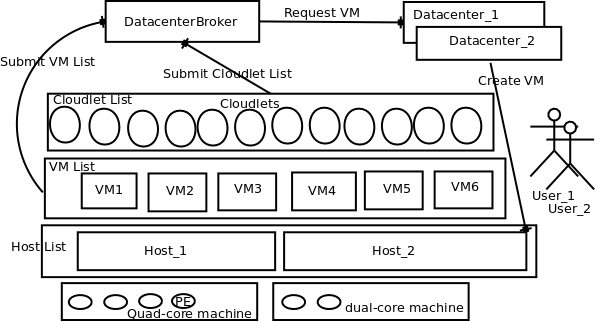
\includegraphics[width=\textwidth]{resources.png}
 }
 \caption{CloudSim scheduling operations}
 \label{fig:scheduling}
\end{figure}
Scheduling of resources are modelled at host and VM levels in CloudSim. At the host level, fractions of the processor element is shared across the VMs running in the host. This is handled by the VmScheduler classes. Similarly, the resources are shared among the cloudlets running in a single VM at the VM level, by the CloudletScheduler classes. Classes ${X|Y}SchedulerSpaceShared$ implement the space shared system using FCFS, where ${X|Y}SchedulerTimeShared$ implement the time shared system using Round Robin. Here, X refers to Cloudlet and Y refers to VmScheduler, which handle the resource allocation at the VM and host level accordingly. The examples and default scenarios often use the TimeShared systems, which use Round Robin algorithm. The application level behaviour, which of the cloudlets from the broker is executed next, is defined at the broker level. However, these policies could be mixed and the algorithm implementations for the application scheduling were tested against these different combinations of scheduling algorithms at VM and host level.

The total number of cloud user entity plays an important role to determine whether all hostList should be shut down or not. The hostList will be shutdown, unless one or more users are still not finished. It is important to give a correct number of total cloud user entity to avoid CloudSim hanging or displaying a weird behaviour.

\SubSection{Scheduling Algorithms at Broker Level}


%------------------------------------------------------------------------- 
\Section{Evaluation}
CloudSim is bundled with examples that could be extended to simulate more complicated scenarios. The existing examples and the user simulations could be executed from the folder $cloudsim-3.1-SNAPSHOT/jars$, using a command similar to the one below.
\begin{verbatimtab}
java -classpath
    cloudsim-3.1-SNAPSHOT.jar:
    cloudsim-examples-3.1-SNAPSHOT.jar 
    org.cloudbus.cloudsim.examples.
    CloudSimExample6
\end{verbatimtab}

Sufferage is the loss that is caused, if the job is not scheduled this time and scheduled to the next available resource instead.

\SubSection{Environment}
The development of experiments and the evaluation were carried on a platform of Ubuntu 12.04 LTS (precise) - 64 bit, Kernel Linux 3.2.0-40-generic and GNOME 3.4.2. The environment had 1.9 GiB memory and Intel\textregistered Core\texttrademark 2 Duo CPU T6600 @ 2.20GHz * 2 processor available. Java(TM) SE Runtime Environment (build 1.6.0\_31-b04)l hardware environments, and work with the simulations.
\SubSection{Configurations}
CloudSim was configured with different configurations of jobs and resources and the experiments are continued to study the behaviour of the scheduling algorithms. Some algorithms started to hang up, in a few upper level conditions, which are marked as the extreme conditions for the given configurations in the environment, and further experiments were conducted ensuring that the extreme conditions are not reached. Testing was carried on with 5 virtual machines and up to 4000 cloudlets. Most of the initial experiments were carried ahead with processing elements of 1000 MIPS, 1 CPU in each virtual machines, while the cloudlets having a length of 1000, file size of 300, output size of 300, pesNumber of 1, and with 2 users.
\begin{figure}[ht]
 \resizebox{\columnwidth}{!}{
  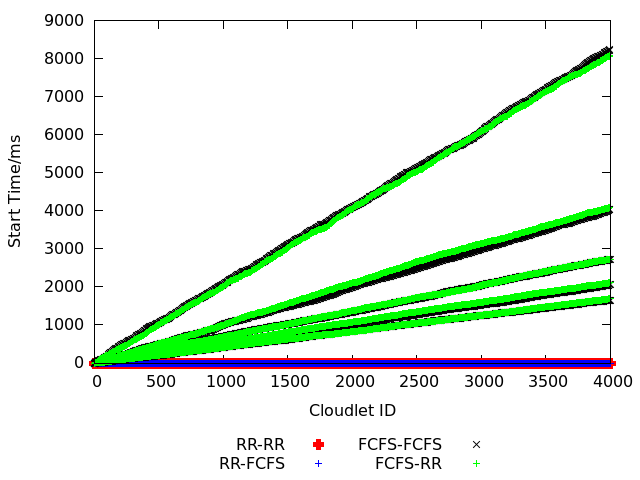
\includegraphics[width=\textwidth]{init5_4000.png}
 }
 \caption{VM and Host level Scheduling Vs Starting Time}
 \label{fig:start}
\end{figure}
\begin{figure}[ht]
 \resizebox{\columnwidth}{!}{
  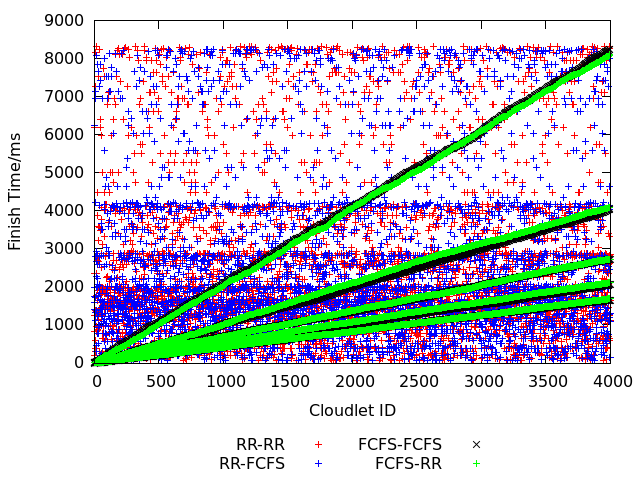
\includegraphics[width=\textwidth]{fin5_4000.png}
 }
 \caption{VM and Host level Scheduling Vs Finishing Time}
 \label{fig:finish}
\end{figure}
Before evaluating the application scheduling algorithms, CloudSim was first tested with the random application scheduling which is the default behaviour of the broker. The space shared schedulers with first-come first-served algorithm and the time shared schedulers with round robin algorithms were tested for both the VM and Cloudlet scheduling. As indicated by Figure 2, all the cloudlets were started almost immediately when host level scheduling was run with round robin. But first-come first-served started in the order the tasks submitted. Round robin effectively shares the time window against the multiple cloudlets. As shown by Figure 3, by switching the available time frame to multiple applications, all the cloudlets tend to finish at the same time regardless of their starting order. However, in first-come first-served, the cloudlets from the VMs that were started finished before the ones that were submitted later. This behaviour ensured that the minimum execution time of first-come first-served was minimized. However, the cloudlets that arrived later had to wait much longer even to have the Pe allocated to them. This increased the starting time or the submission time. The observations indicate that the host level scheduling is dominating in starting and finishing time.

To avoid influencing the application scheduling with these multiple scenarios involving these host level and VM level scheduling, TimeShared policies with round robin algorithm were used at these levels for evaluating the application scheduling at the broker level.
\SubSection{Results}

%------------------------------------------------------------------------- 
\Section{Conclusion}
Strictly matchmaking-based algorithms focus to optimize a specific objective function. User's satisfaction depends on how much of his multiple requirements are satisfied by the scheduling algorithms. User utility was proven to be reasonably high for all the criteria considered for the utility based algorithm developed considering the partial requirements satisfaction. QoS based algorithm too performed reasonably high in the evaluation criteria. Hence it is mandatory to develop efficient utility based scheduling algorithms for a cloud environment involving multiple user applications and multiple resources that have to satisfy the users with heterogeneous evaluation criteria.

While criteria such as minimum execution time and minimum completion time could be a good start for evaluating the scheduling algorithms, many other parameters take higher precedence in a real cloud environment. Evaluation criteria could be developed based on the market requirements such as the cost of the cloud resource. QoS-based algorithms focus on such priorities. Developing effective evaluation criteria is essential for measuring the user satisfaction with a considerable accuracy. The effectiveness of the simulation environment to depict the real cloud scenarios is still a question to be addressed. While it is sufficient to test the prototypes and the algorithms against the simulation environment during the early phases of development, it is essential to test the production-ready algorithms against the real cloud deployments.
%------------------------------------------------------------------------- 
\Section{Acknowledgements}

My special thanks goes to Prof. Luiz Veiga for his continuous motivation and assistance in this project as this is highly relevant to my thesis. As a project that is heavily used by the researchers and academics in their projects and research activities, CloudSim project mailing list is always active with a vibrant community. I am grateful to the original developers and the community of CloudSim as well as the researchers who were the authors of the respective scheduling algorithms.

%------------------------------------------------------------------------- 
\Section{References}


%------------------------------------------------------------------------- 
\nocite{ex1,ex2}
\bibliographystyle{cloudsim}
\bibliography{cloudsim}

\end{document}

